\documentclass[UTF8]{article}

%--
\usepackage{ctex}
\usepackage[margin=1in]{geometry}
\usepackage{amsmath}
\usepackage{amssymb}
\usepackage{graphicx}
\usepackage{graphics}
\usepackage{float}

%--
\begin{document}
    
%--
{\flushleft \bf \Large 姓名:} 杨佩成

{\flushleft \bf \Large 学号:} MG1733079

{\flushleft \bf \Large 日期:} 2017.12.10


%=========================================================================
\section*{论文信息}
    
L. Lamport, Time, clocks, and the ordering of events in a distributed system. Communications of the ACM. 21, 558–565 (1978).


%=========================================================================
\section{概述}

	分布式系统是一组不同进程的集合,这些进程在空间上是分离的并且通过交换消息来进行通信。在分布式系统中,有时很难确定两个事件中哪个先发生。“happen before”关系只是整个系统中的一个偏序。这篇文章讨论了用“happened before”定义的偏序,并提出一个将偏序扩展到系统全序的算法。我们利用系统的全序关系可以解决分布式系统中的同步问题。但是因为系统的全序并不是唯一的,可能会产生一些异常行为,这些异常行为可以通过引入物理时钟来避免。

\section{偏序与全序}

	偏序指的是系统中部分事件的先后顺序。在分布式系统中我们有时无法确定系统中哪个事件先发生,我们只能通过“happened before”关系推出系统中的偏序关系。

	我们假设系统由一组进程组成,每个进程是一组有序事件的集合,发送消息和收到消息也是事件。我们用“$\to$”来表示两个事件的“happened before”关系。

	定义:(1)若$a$和$b$是用一个进程中的两个事件,并且$a$在$b$之前发生,则$a \to b$。

		(2)若$a$和$b$在两个不同的进程中,$a$是一条消息的发送方,$b$是同一条消息的接收方,则$a \to b$。

		(3)若$a \to b$,$b \to c$,则$a \to c$。若$a \nrightarrow b$,$b \nrightarrow a$,则称事件$a$和$b$是同步的。

	如图1,水平方向代表空间,垂直方向代表	时间,越高代表时间越靠后。点表示事件,垂直的线表示进程,曲线表示消息。$a \to b$表示在一个进程上$a$在$b$之前或者在一条曲线上上$a$指向$b$。我们还可以把$\to$理解为因果关系,如果$a \to b$则可以认为$a$是$b$发生的原因。
\begin{figure}[H]
\centering
\small
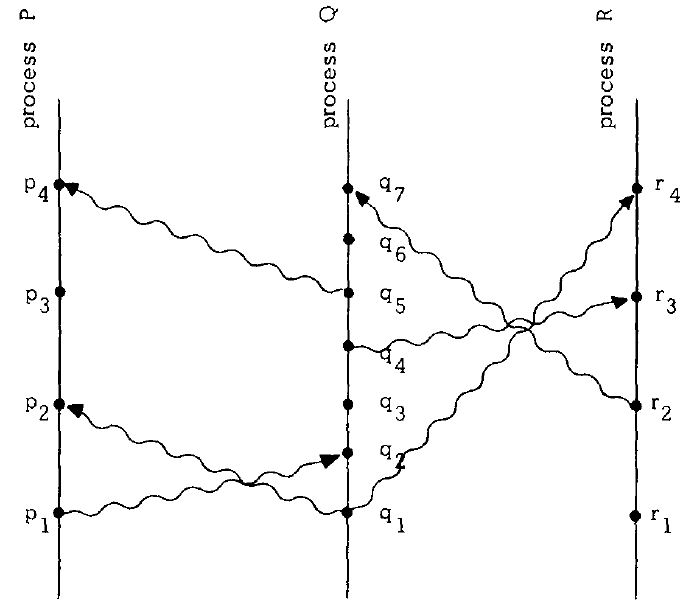
\includegraphics[width=10cm,height=10cm]{1.JPG}
\caption{时空图}
\end{figure}
	
	我们在“happened before”的基础上定义系统的逻辑时钟。我们通过给每个事件分配一个数字来给系统引入时钟。给每一个进程$P_i$定义一个时钟$C_i$,$C_i$实际上是一个函数,$C_i \langle a \rangle$表示进程$P_i$给事件$a$分配的数字。整个系统的时钟用函数$C$表示,系统给事件$b$分配的数字表示为$C \langle b \rangle$。若$b$是进程$P_j$中的事件,则$C\langle b\rangle =C_j\langle b\rangle$。在这个定义中$C_i$与物理时钟无关,所以我们可以认为$C_i$是系统的逻辑时钟。因为在逻辑时钟定义中没有涉及物理时间,所以我们时钟定义的正确性必须基于事件发生的顺序。我们定义的时钟条件如下,
	
	$Clock \quad Condition. \quad$对于任意事件$a$,$b$,若$a \to b$,则$C \langle a \rangle < C \langle b \rangle$。
	
	只要下面两个条件满足,时钟条件就可以满足,
	
	$C1$.\quad若$a$和$b$是进程$P_i$的两个事件,$a$在$b$之前发生,则$C_i \langle a \rangle < C_i \langle b \rangle$。

	$C2$.\quad若$a$在进程$P_i$中,$b$在进程$P_j$中,$a$是一条消息的发送方,$b$是同一条消息的接收方,则$C_i \langle a \rangle < C_j \langle b \rangle$。

	我们假设进程$P_i$的时钟用寄存器$C_i$表示,$C_i \langle a \rangle$表示$C_i$在事件$a$期间的值。$C_i$的值在不同事件期间会改变,$C_i$值的变化本身并不构成事件。如果要在实际系统中引入时钟并且保证时钟能够满足时钟条件,只需要满足以下实现规则:

	$IR1$.\quad每个进程$P_i$维护一个$C_i$,并且当有新的事件发生时,$C_i$加一。

	$IR2$.\quad$(a)$进程$P_i$中的事件$a$在发送信息$m$时,会包含一个时间戳$T_m$,$T_m$等于$C_i \langle a \rangle$。
		 \quad$(b)$当进程$P_j$收到消息$m$后,$P_j$会更新$C_j$,保证$C_j$大于等于当前值并且大于$T_m$。

	规则$IR1$保证了系统满足$C1$,$IR2$保证了满足$C2$。因此只要系统满足了上述的规则,就可以保证系统有一个正确的逻辑时钟。

	在系统中引入时钟,我们就可以对系统中的所有事件进行排序(只需要按照它们发生的时间进行排序),得到系统的全序。为了打破系统中可能的同步关系,我们在进程之间引入任意的顺序关系$\prec$,这样我们就可以定义系统的全序关系$\Rightarrow$:
	
	$a$是进程$P_i$中的一个事件,$b$是进程$P_j$中的一个事件,若$(\romannumeral1)C_i\langle a \rangle < C_j \langle b \rangle$或$(\romannumeral2) C_i\langle a \rangle = C_j \langle b \rangle$并且$P_i \prec P_j$,则$a \Rightarrow b$。

	从全序关系的定义和时钟条件可以证明如果$a \rightarrow b$,则$a \Rightarrow b$。全序关系依赖于系统的时钟,并且系统的全序关系是不唯一的,因为我们在不同进程之间引入的顺序关系是任意的。不同的时钟,只要满足了时钟条件,就可以生成不同全序。在分布式系统中,只有偏序是唯一的。

	在分布式系统中引入逻辑时钟,可以得到一个系统的全序。通过全序,我们可以解决一类互斥问题。

	基本问题:在一个分布式系统中,有一组固定的进程共享一个资源。在每个时刻只能有一个进程能够使用这个资源。分配资源的算法必须满足下面三点要求:(1)资源在被分配给新的进程之前必须先被旧的进程释放。(2)资源的分配顺序必须和进程的请求顺序一致。(3)每个获取了资源的进程最终都会释放资源,每个请求最终都会得到授权。
	
	使用一个集中调度的进程来处理资源分配在一些情况下会失效。假设$P_0$是调度进程,$P_1$先给$P_0$发送一个资源授权请求,再给$P_2$发送一个消息。$P_2$在收到消息后也发送一个请求给$P_0$。如果$P_2$的请求先到达,那么上面的条件3就会不满足。
	
	我们可以在系统中引入逻辑时钟来解决这个问题。为了简化问题,我们假设两个进程之间消息的到达顺序与发送顺序一致,每个消息最终都能被收到,每个进程都能与其他任一进程通信。每个进程都维护一个仅自己可见的请求队列,初始情况下队列只有一条消息$T_0:P_0$请求资源。$P_0$是最初被授予资源的进程,$T_0$小于任意时钟初始值。具体算法由下面五条规则定义:

	1.当进程$P_i$请求资源时,它会向其它进程广播$T_m:P_i$请求资源的消息并把消息加入自己的请求队列中,其中$T_m$是发送消息的时间戳。

	2.当进程$P_j$收到$T_m:P_i$请求资源的消息时,它会将消息放入自己的请求队列中并回复一个带时间戳的$ack$给$P_i$。

	3.若$P_i$要释放资源,它会将$T_m:P_i$请求资源的消息从自己的请求队列中删除,并向其它进程广播一个带时间戳的释放资源的消息。

	4.当进程$P_j$收到来自$P_i$的释放资源消息时,它会从请求队列中将$T_m:P_i$请求资源的消息删除。
	
	5.当下面两个条件满足时,进程$P_i$会被授予资源:$(\romannumeral1)$在它自己的消息队列中,不存在比$T_m:P_i$更早的请求资源消息,这里的顺序通过全序定义的。$(\romannumeral2)$$P_i$发送的请求收到其它进程的回复。

	我们可以证明这个算法能够满足问题的三点要求。规则5的$(\romannumeral2)$和进程有序接收的假设,可以保证$P_i$可以知道所有请求的先后顺序。规则3和规则4能够从请求队列中删除消息,这可以保证问题的要求1可以满足。要求2通过系统的全序满足。规则2保证了在$P_i$请求资源后,规则5的$(\romannumeral2)$最终会成立。规则3和4保证了每个获得了资源的进程最终会释放资源,然后规则5的$(\romannumeral1)$就会成立。

	这是一个分布式的算法,不需要中心节点,每个进程都各自按照这套规则执行。这种算法可以实现分布式系统中的任何同步操作。因为所有的进程都是按照时间戳(由系统的全序决定)来执行命令的,每个进程都是执行的一个相同的命令序列。但是这种算法需要所有的进程都积极参与,当一个进程发生故障时,其它进程就不能继续执行命令,这会导致整个系统的停止。如果没有物理时钟,我们是无法区分进程故障和进程暂停的。

\section{异常行为与物理时钟}

	我们的资源调度算法是通过系统的全序来对请求排序,这就存在发生异常行为的可能。假设一个人在计算机A上提出一个请求A,然后打电话给一个朋友让他在电脑B上提出一个请求B,系统很有可能先对B进行响应。系统并不知道A在B之前发生,因为这个先后顺序信息是基于系统外部消息的。假设$\varphi$是系统内部所有事件的集合,\underline{$\varphi$}是系统内部事件和与内部事件相关的外部事件的并集。我们用$\boldsymbol{\rightarrow}$表示\underline{$\varphi$}中的“happened before”关系。$A \boldsymbol{\rightarrow} B$不能推出$A \rightarrow B$。因为我们不能保证从系统的内部事件能推出A在B之前发生。有两种可能的方式可以用来避免这种异常行为,第一种方式是在系统中引入关于$A \boldsymbol{\rightarrow} B$的相关信息。第二种方式是在系统中构建一个满足强时钟条件的时钟。强时钟条件是指对于$\varphi$中的事件$a$和$b$,如果$a \boldsymbol{\rightarrow} b$,则$C\langle a \rangle < C\langle b\rangle$。我们可以引入物理时钟来满足强时钟条件,从而消除系统中的异常行为。

	我们用$C_i(t)$表示时钟$C_i$在物理时刻$t$的读数。我们假设时钟是连续的,并且除非时钟重置,$C_i(t)$是连续可导的。$\frac{dC_i(t)}{dt}$表示时钟在$t$时刻的变化速率。如果$C_i$要是真实的物理时钟,需要满足下面两点条件:

	$PC1.$ $\quad$ 存在一个常数$\kappa \ll 1$,对任意的$t$,$|\frac{dC_i(t)}{dt}-1|<\kappa$.

	$PC2.$ $\quad$ 对任意$i$和$j$,$|C_i(t)-C_j(t)|<\epsilon$.

	$PC1$保证了$C_i$可以以一个正确的速率运转,$PC2$要求不同时钟之间是同步的。但是由于不同时钟不会按照一个严格相同的速率运行,它们会趋向于误差越来越大。所以必须设计一个保证$PC2$一致成立的算法。我们基于逻辑时钟中的$IR1$和$IR2$设计了物理时钟的实现规则:
	
	$IR1'.$ \quad 对于任意$i$,如果$P_i$在物理时刻$t$没有收到消息,那么$C_i$在$t$时刻就是可导的,并且$\frac{dC_i(t)}{dt}>0$.

	$IR2'.$ \quad $(a)$如果$P_i$在物理时刻$t$发送了消息$m$,那么$m$中就会包含一个时间戳$T_m=C_i(t)$。$(b)$如果$P_j$在时刻$t'$收到消息$m$,$P_j$就会将$C_j(t')$设置为$C_j(t'-0)$和$T_m+\mu_m$中的最大值,其中$\mu_m$为通信的最小延时。

\section{总结}
	本文基于“happened before”的概念定义了分布式系统中的偏序关系,提出了一个将偏序扩展到全序的算法,并利用全序解决了一个同步问题。在分布式系统中,只有偏序是确定的,全序是并不是唯一的,这会导致系统中异常行为的产生,异常行为可以通过同步物理时钟来消除。
	
	这篇文章中的一个重要观点是我们时空中的事件并不存在一个唯一的全序关系,不同的观察者对事件发生的先后顺序会有不同的看法。只有当事件$e2$是由事件$e1$引起时,事件$e1$和$e2$才会存在一个唯一的先后顺序。通过定义一个系统的全序,我们理论上可以实现任意的分布式系统。一个分布式系统可以描述为一个特殊的具有多个由网络互联的处理器的串行状态机。如果能对输入请求全排序,就能实现任何由网络互联处理器组成的状态机,因此也就能实现任意的分布式系统。
	

%--
\end{document}